\begin{figure}[tb]
\center{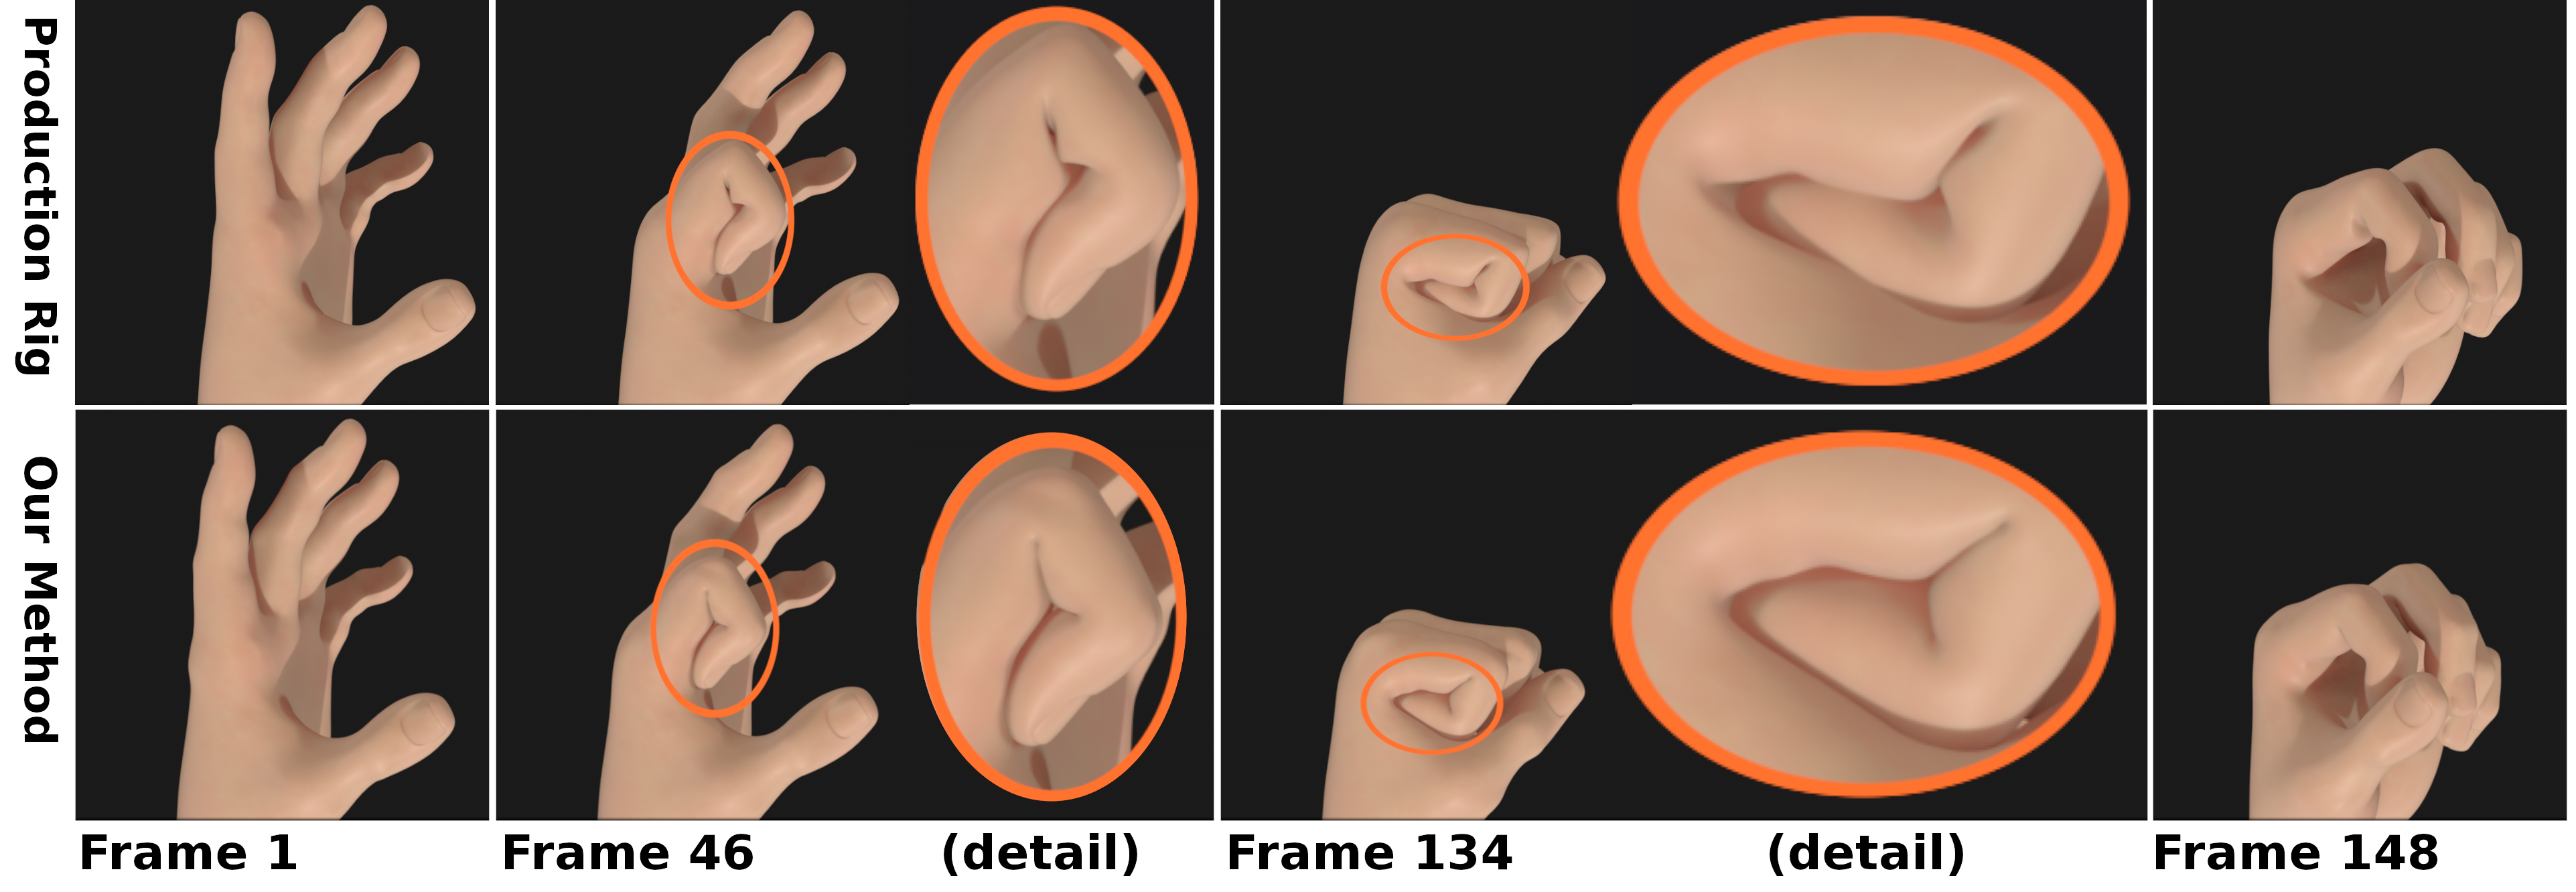
\includegraphics[width=1\linewidth]{elasticity/figures/handfigure}}
\caption[A hand rigged using linear blend skinning and our method.]{Top: A hand rigged using linear blend skinning. Due to the many joints
it is impractical to model all the shapes necessary fix the artifacts using an
example based technique like PSD. To compensate, a significant amount of effort was
spent on creating a nice skin bind for this hand. Bottom: The same hand rigged with our
elasticity based deformer using 117,607 non-empty cells. Note how we get correct creasing and contact
deformation where the finger bends.}
\label{fig:hand}
\end{figure}


\paragraph{Initial guess.} A very significant source of optimization is the choice of initial guess because
we use iterative methods.  To make solutions deterministic and completely frame
independent we considered the use of a base linear blend skin as an initial
guess. However, this can lead to unstable behavior in the presence of large
contact deformations because collision resolution is path dependent. Instead, we therefore use the previous
solution (often the previous frame) as an initial guess. 

\paragraph{CPU.} To improve performance on the CPU we utilized multithreading using a task
queue. We designed our access patterns to be cache friendly by using blocking
techniques.  We also exploited SSE data level parallelism for the SVD
computation. Additionally, we used templatization to optimize stride
multiplication computations in array accesses. Constraint contributions to the
matrix were baked into a structure that minimized indirection.

\paragraph{GPU.} Since GPUs have become popular for parallel numerical algorithms, we did a
na\"{i}ve port of our CPU oriented code to the GPU. Our expertise at optimizing
for the GPU's different bandwidth versus computation tradeoffs was limited, and
we hope to utilize the grid optimization techniques of \cite{Dick:2011:CUDAFEM}
in the future.

We benchmarked our elasticity multigrid solver on a cube model with Dirichlet constraints on two opposite faces without collisions or point constraints. While we were able to attain a
convergent method with as few as 2 Jacobi smoothing sweeps per grid transfer, we were able to achieve the best balance between speed and convergence rate with 5-10 Jacobi relaxation
sweeps.  In all cases, the first V-cycles significantly (by 1-2 orders of magnitude) lowered the residual before settling into a constant convergence rate between 0.5 and 0.75, depending
on the number of relaxation sweeps.
On a $32\times32\times32$ element cube, we averaged 0.031s on the GPU and 0.10s on the CPU  per V-cycle with 10 relaxation
sweeps per grid transfer on 4 levels.  On a $64\times64\times64$ element cube, we averaged 0.086s on the GPU and 0.56s on the CPU per V-cycle with 10 relaxations sweeps on 5 levels.  In practice, we found that 1-2
V-cycles were sufficient for the Newton-Raphson solver to converge.

\subsection{Diagonal part of stiffness matrix}

The Jacobi iteration used as the smoother in our multigrid scheme requires explicit knowledge of the diagonal part of the stiffness matrix $\mathbf{K}$. Since we never construct this
matrix explicitly, a specialized process needs to be followed to compute the diagonal part directly and efficiently. 

For element $\Omega_e$ we will define the contribution of each of the 24 degrees of freedom to the diagonal
part of $\mathbf{K}$. In particular, we turn our attention to the degree of freedom $x_i^{(j)}$, that is the $j$-th component of the $i$-th element vertex, where
$i\in\{1,\ldots,8\}$ (see Figure~\ref{fig:cubic_element}). 

Also, define $\vec{g}$ to be the $i$-th \emph{column} of the discrete gradient $\mathbf{G}$, and $\vec{r}^T$ the $j$-th \emph{row} of $\mathbf{R}$. Also, define
$\mathbf{M}_i=\mathcal{E}:\vec{g}$ (i.e.\ the right-side cross product matrix with $\vec{g}$). Also define
$
\mathbf{N}_i=\lambda\vec{g}\vec{g}^T+\mathbf{M}_i^T\mathbf{L}\mathbf{M}_i.
$
where $\mathbf{L}$ was defined in section \ref{sec:indefiniteness}. The diagonal contribution of $\Omega_e$ to the diagonal part corresponding to degree of freedom $x_i^{(j)}$ is
$
\hbox{\small$\frac{3}{2}$}\mu/h^2+\vec{r}^T\mathbf{N}_i\vec{r}.
$
We can verify that the diagonal entries corresponding to antidiametric vertices (e.g. $\vec{x}_1$ and $\vec{x}_8$) are equal; thus the diagonal entry need only be computed for the
components of 4 out of the 8 vertices of the element. Finally $\mathbf{N}_i$ can be precomputed, we only need to consider $i=1,\ldots,4$ as we explained, and these matrices are
identical for all elements. 

\subsection{Fast Singular Value Decomposition}

Our method makes use of the Singular Value Decomposition $\mathbf{F}=\mathbf{U\Sigma V}^T$ to define the matrix $\mathbf{L}$, and in fact we use it to construct the rotational factor of
the Polar Decomposition as well, as $\mathbf{R}=\mathbf{UV}^T$. The cost of the $3\times 3$ SVD is commonly acknowledged as a bottleneck for corotational or shape matching methods. We
introduce a new, and highly efficient methodology which is virtually branch-free (other than the use of conditional assignments, which is an atomic instruction in SSE4.1 and other
platforms), uses no expensive arithmetic other than addition, subtraction, multiplication and an \emph{inexact} square root (i.e. the SSE $VRSQRTPS$ instruction), and is trivially
and extensively vectorizable. We ultimately obtain a cost per decomposition equal to $11$ns on a 12-core X5650 workstation, using SSE and multithreading in conjunction. This cost is
about 1/40 of recently reported results \cite{Rivers:2007:FFL}, and we require the exact same computation for \emph{any} matrix, without counting on warm starts for acceleration.

The core cost of the SVD analysis is commonly reported to be the symmetric eigenanalysis. An iterative Jacobi diagonalization procedure is often used to bring the symmetric matrix
$\mathbf{S}=\mathbf{F}^T\mathbf{F}$ into diagonal form. Instead of the exact Givens conjugation used in the Jacobi procedure, we define an \emph{approximate} Givens angle, which can be obtained
with minimal computation. The optimal Givens angle that annihilates element $s_{21}$, for example is known to satisfy $\tan(2\theta)=2s_{12}/(s_{11}-s_{22})$. Instead of using an inverse
trigonometric function (or the alternative approach of solving a quadratic equation), we consider the following asymptotic approximation, valid when $\theta$ is small:
$$
\frac{2s_{12}}{s_{11}-s_{22}}=\tan(2\theta)\approx 4\tan(\frac{\theta}{2})\Rightarrow\frac{\sin(\theta/2)}{\cos(\theta/2)}\approx\frac{s_{12}}{2(s_{11}-s_{22})}
$$
At this point, we observe that this approximate rotation can be stored as the un-normalized quaternion $(2(s_{11}-s_{22}),0,0,s_{12})$, eliminating the need for divisions or exact
normalizations. In fact, we do perform an \emph{inexact} normalization using the approximate $VRSQRTPS$ SSE instruction, merely for the purpose of avoiding overflow, and without this
inaccuracy affecting the semantics of the quaternion. However, the asymptotic approximation does not hold for arbitrary $\theta$, and it would be possible that the off-diagonal element
would not be reduced (let alone, annihilated) for certain cases. However, we can show that the best of either the above approximation \emph{or} a choice of $\theta=\pi/4$ is guaranteed
to reduce the magnitude of the off diagonal element $s_{12}$ by at least a factor of $0.6$ per application. Deciding which one to use is made with a simple algebraic check, as shown in Algorithm \ref{alg_approx2}.
\begin{algorithm}[h]
\caption{Computation of approximate Givens quaternion.}
\label{alg_approx2}
\begin{algorithmic}[1]
\State \textbf{const} $\gamma\gets 3+2\sqrt{2}$, $c_\ast\gets \cos(\pi/8)$, $s_\ast\gets \sin(\pi/8)$
\Function{ApproxGivensQuaternion}{$a_{11},a_{12},a_{22}$}
\State $c_h\gets 2(a_{11}\!-\!a_{22})$\Comment{$c_h \approx \cos(\theta/2)$}
\State $s_h\gets a_{12}$\Comment{$s_h \approx \sin(\theta/2)$}
\State $b\gets[\gamma s_h^2<c_h^2]$\Comment{$b$ is boolean}
\State $\omega\gets \texttt{RSQRT}(c_h^2+s_h^2)$\Comment{$\texttt{RSQRT}(x)\approx 1/\sqrt{x}$}
\State $c_h\gets b$\texttt{?}$\omega c_h$\texttt{:}$c_\ast$
\State $s_h\gets b$\texttt{?}$\omega s_h$\texttt{:}$s_\ast$
\State \Return $(c_h,0,0,s_h)$\Comment{returns a quaternion}
\EndFunction
\end{algorithmic}
%\vspace{-15pt}
\end{algorithm}

%\vspace{-20pt}
Once the matrix $\mathbf{S}$ has been brought closer to a diagonal, our asymptotic approximation becomes extremely accurate, and essentially matches the efficiency of regular Jacobi
iteration (but at a fraction of the implementation cost). We have invariably observed that 4 sweeps of our method offer the same efficacy in diagonalizing $\mathbf{S}$ as 3 sweeps of the
regular Jacobi method, and this brings the magnitude of off-diagonal entries to 4-5 order of magnitude smaller than the singular values on the diagonal. Once the symmetric eigenanalysis
has been computed, we robustly compute the rotational factor $\mathbf{U}$ by performing a Givens $\mathbf{QR}$ factorization on $\mathbf{AV}=\mathbf{U\Sigma}$, which generates an exactly
orthogonal factor $\mathbf{Q}=\mathbf{U}$ and a triangular factor $\mathbf{R}$ which will in fact be \emph{diagonal} (and equal to $\mathbf{\Sigma}$) as long as the columns of
$\mathbf{U\Sigma}$ are sorted in descending order of magnitude by permuting them along with the columns of $\mathbf{V}$. The Givens QR factorization has a completely deterministic
control flow, and can also be highly vectorized. We refer the interested reader
to the supplemental technical document for full analysis and implementation.

%  a robust mathematical analysis of our proposed method, and
%detailed implementation instructions. 
